%Special Track: Special Session on Human-centric Internet and Multimedia Systems
%Topic: User-centric algorithms in multimedia systems covering
%Deadline: 15/12/2017


\documentclass[sigconf]{acmart}

\usepackage{booktabs} % For formal tables


% Copyright
%\setcopyright{none}
%\setcopyright{acmcopyright}
%\setcopyright{acmlicensed}
%\setcopyright{rightsretained}
%\setcopyright{usgov}
%\setcopyright{usgovmixed}
%\setcopyright{cagov}
%\setcopyright{cagovmixed}


% DOI
%\acmDOI{10.475/123_4}

% ISBN
%\acmISBN{123-4567-24-567/08/06}

%Conference
%\acmConference[MMSys'2018]{ACM Woodstock conference}{July 1997}{El
 % Paso, Texas USA} 
%\acmYear{1997}
%\copyrightyear{2016}


%\acmArticle{4}
%\acmPrice{15.00}

% These commands are optional
%\acmBooktitle{Transactions of the ACM Woodstock conference}
%\editor{Jennifer B. Sartor}
%\editor{Theo D'Hondt}
%\editor{Wolfgang De Meuter}


\begin{document}
\title{CrowdNote: Turning Wisdom and Effort of Crowds into Complex Media  Annotation}

\author{Marcello N. de Amorim}
\affiliation{%
  \institution{Federal University of Esp\'irito Santo}
}
\email{novaes@inf.ufes.br}

\author{F\'abio R. de A. Neto}
\affiliation{%
  \institution{Federal University of Esp\'irito Santo}
}
\email{fabio.ribeiro.neto@gmail.com}

\author{Celso A. S. Santos}
\affiliation{%
  \institution{Federal University of Esp\'irito Santo}
}
\email{saibel@inf.ufes.br}


% The default list of authors is too long for headers.
\renewcommand{\shortauthors}{Marcello N. de Amorim et. al.}


\begin{abstract}
	Media annotation consists of supplementing media objects, such as videos, images, and audios, by adding metadata about their content and context, also to describing media characteristics such as quality, encoding, among other features. Complex media annotation involves annotating different aspects of media objects as well as relating them. This kind of annotation usually is associated with a demanding process that requires experts and elaborated annotation system. This paper presents a method to achieve complex media annotation without requiring complex tools, experts nor trained workers. In this method, the complex annotation process is divided into a set of simple annotation microtasks, and based on them is defined a process workflow for generating complex annotation. To demonstrate the operation of this method, we developed a video enrichment system and carried out an experiment in which the crowd was responsible for executing a set of simple annotation microtasks through simple tools. 



\end{abstract}

\begin{CCSXML}
<ccs2012>
<concept>
<concept_id>10002951.10003260.10003282.10003296</concept_id>
<concept_desc>Information systems~Crowdsourcing</concept_desc>
<concept_significance>500</concept_significance>
</concept>
<concept>
<concept_id>10003120.10003130.10003131.10003570</concept_id>
<concept_desc>Human-centered computing~Computer supported cooperative work</concept_desc>
<concept_significance>500</concept_significance>
</concept>
<concept>
<concept_id>10010405.10010497.10010510.10010513</concept_id>
<concept_desc>Applied computing~Annotation</concept_desc>
<concept_significance>500</concept_significance>
</concept>
<concept>
<concept_id>10002951.10003227.10003251</concept_id>
<concept_desc>Information systems~Multimedia information systems</concept_desc>
<concept_significance>500</concept_significance>
</concept>
<concept>
<concept_id>10003120.10003121.10003124.10010868</concept_id>
<concept_desc>Human-centered computing~Web-based interaction</concept_desc>
<concept_significance>500</concept_significance>
</concept>
</ccs2012>
\end{CCSXML}

\ccsdesc[500]{Information systems~Multimedia information systems}
\ccsdesc[500]{Human-centered computing~Web-based interaction}
\ccsdesc[500]{Information systems~Crowdsourcing}
\ccsdesc[500]{Human-centered computing~Computer supported cooperative work}
\ccsdesc[500]{Applied computing~Annotation}


\keywords{Crowdsourcing, Media Annotation, Video Annotation, Human Computation, Microtasks, Multimedia Systems, Video Enrichment}


\maketitle

\pagebreak
\section{Introduction}
	Media annotation consists of supplementing media objects, such as videos, images and audios, by adding metadata about their content and context,  also to describing media characteristics such as quality, encoding, among other features \cite{Wang:2009:BDM:1652990.1653002}. This supplementary information can be used to make easier the work of users and systems that can handle annotated items \cite{172450}. It allows highlighting key points as well as add information to content presented\cite{Cunha:2015:MVA:2820426.2820449}, facilitating the creation of media applications for content-based distribution \cite{Zhang:2012:KIE:2339530.2339620}, indexing \cite{Zhang:2007:PRS:1290082.1290126}, summarization \cite{Fiao:2016:AGS:3001773.3001802}, navigation \cite{Goldman:2008}, composition \cite{Wilk:2015:VCC:2713168.2713178}, among many others, by both automatic and manual means \cite{Wang:2011:ALM:1899412.1899414,Mihalcea:2007:WLD:1321440.1321475}. 

In this paper, media annotations are categorized as simple and complex ones, considering that simple annotations are those that can be acquired with a simple interaction of the workers in a microtask. Complementarily, a complex annotation is one that requires the worker execute a more tedious, hard or time-consuming task, in which he needs to perform multiple interactions. 

Automatic methods for media annotations often present satisfactory efficiency and interesting results, though, they generally apply techniques that require well-structured media objects and extensive examples database, such as deep learning\cite{lecun2015deep}. Unfortunately, many scenarios cannot provide these requirements, making it impossible to use automatic methods for video annotation \cite{murthy2015automatic}. 

In another way, manual media annotation is suitable for these scenarios because it uses human intelligence to handle the tasks. However, manual video annotation can be high-costly because of the potentially high-density of annotation points in the video, as well as the complex nature of some annotation tasks. 

An alternative to achieving a media annotation in a general scenario is to employ collaborative or cooperative approaches, which are differentiated in this paper. In a collaborative approach, the contributors work together to solve the main problem. Otherwise, in a cooperative approach, each contributor solves a part of the main problem to produce a final result \cite{misanchuk2001building}.

Taking cooperative approaches to a higher level, crowdsourcing media annotation has emerged as a proposal to annotate media objects using a large number of contributors efficiently \cite{VonAhn:2005:HC:1168246}. Following the crowdsourcing principles, the tasks distributed to the workers are modeled to be done independently, maximizing the parallelism \citep{Howe2006}. Moreover, each task can be sent to many contributors, making possible to compare, check and to aggregate the contributions also reducing the chance of producing a biased result \cite{GALTON1907}.

A frequent problem of using a crowdsourcing approach to media annotation is to balance the relationship between task complexity and cost. Simple annotation tasks, such as clicking an object on a video, can be done in a few seconds for anyone. Otherwise, more complex tasks such as providing complementary content and positioning it in the right position on a video, require some expertise of contributors and are more costly to them. In a crowdsourcing context, microtask is a ubiquitous designation for simple tasks that can be performed for any contributor quick and easily \cite{Difallah:2015:DMC:2736277.2741685}.

The method presented in this paper aims to achieve a complex media annotation without requiring trained workers or experts, employing a set of simple annotation tools rather than complex and expensive annotation systems. In this way, a complex annotation process is divided into a set of simple annotation microtasks, and based on them is defined a workflow to generating the outcome. This aims to provide ways to get around some problems faced in achieving a complex media annotation:

\begin{itemize}

\item By using manual annotations, no example bases or restricted conditions are required as in automatic methods.

\item By using a microtask-based crowdsourcing process is not required experts nor trained workers. Also, it makes the contribution process simple and quick, avoiding time-consuming and tedious tasks to workers.

\item By using microtasks in which only a simple annotation is collected is not required sophisticated annotation tools.
\end{itemize}


%This paper presents an updated version of CrowdNote, with improvements that made it more flexible and useful by overcoming some important limitations detected in the previous version. The main limitations addressed were:
%\begin{itemize}

%\item Only videos was annotated.

%\item Only supported linear workflows was supported.

%\item The output from each microtask process was designed specifically to use as input to the next microtask.

%\item Only automatic aggregation methods was supported.
%\end{itemize}

Following this method, each simple annotation microtask is modeled here as a process composed by two step: Collection and Aggregation. In the Collection step the contributions are received from the crowd, and in the Aggregation step these  contributions are processed in order to generate its output. 

Also, each microtask is treated as a human computation function, producing an output that can be used as input to the next one in the workflow. In this way, the complex annotation production workflow is treated as a human computation algorithm. This point of view allows to design some features such as generate multiply outputs from a microtask to create simple outcomes from each partial result. These outcomes can be datasets, sumaries, marks and more, so a complex annotation process can generate multiple output artifacts.

A previous version of the method, called CrowdNote, was introduced with some limitation \citep{172450}. This updated version of CrowdNote has incorporated the human computation algorithm concept, which allows to create more flexible production workflows and to produce multiple outputs for each microtask. The scope of the method has also been expanded, including annotations for various media types instead of just videos.

This version also supports automatic, manual and supervised aggregation methods, instead, only automatic ones. Supervised methods are specially useful when is not possible specify rules or algorithms to generate an output from the contributions, this usually involves subjectivity, emotions and other human abilities.

To demonstrate the operation of the method was developed a video enrichment system that was built over a flexible architecture that can handle contributions from internal groups, public groups, and platforms such as Amazon Mechanical Turk, Crowdflower, and Microworkers. Then, an experiment was conducted in which the crowd was responsible for:
\begin{itemize}
\item Identify the points of interest.
\item Suggest extra content.
\item Select the best content for each point of interest.
\item Position them in the scenes. 
\end{itemize}

The rest of this paper is structured as follows. Section 2 presents the concepts used and how they are employed in the proposed approach. Section 3 presents related works. Section 4 presents the extended CrowdNote method and framework. Section 5 presents the conducted experiment. Finally, section 5 concludes the paper presenting final considerations and future prospects.

\section{Related Concepts}
	The presented method is based on the human computation paradigm \citep{VonAhn:2005:HC:1168246}, using a crowdsourcing approach \citep{Howe2006} to annotate media objects. To do so, this method employs some fundamental concepts commonly associated with human computation. These concepts are presented in this section.
%, and it is explained how they are incorporated into the method.

%Its goal is to generate complex annotations without the need for experts nor sophisticated annotation tools. In this method, complex annotations are generated by a composition of simple annotation tasks, which must be modeled so that they can be performed by individuals from a crowd of workers.



	\subsection{Human Computation}
	There are jobs that are trivial for all people, even for kids, but they are extremely difficult even for the most powerful and sophisticated software and software. This type of task has as its characteristics the need for creativity and level of abstraction which, in the present moment, is slightly in the minds of human beings. 

Some examples classify this type of task with image recognition, especially when there is occlusion or involves subjective analysis, content authorship, analysis of emotions and so many other activities that inherently require human intelligence to be performed. Luis von Ahn introduced in his dissertation  \cite{VonAhn:2005:HC:1168246}  a paradigm named Human Computation that allows to approach the problems from this point of view, identifying in it what tasks can be automated and which are those that require human treatment. Additionaly Human Computation can improve performance by division of labor because it helps to define tasks that can be executed in parallel \cite{Rohwer:2010:NHC:1837885.1837897}.

One of the benefits of modeling a system according to the Human Computation paradigm is to focus the effort of human collaborators only on tasks that really require their attention, this is done by identifying the tasks that inherently require human intelligence. Each of these tasks is a HIT (Human Intelligence Task) and corresponds to something that humans can easily solve while a machine presents extreme difficulty in trying to solve \cite{doi:10.2200/S00371ED1V01Y201107AIM013}. 

In short, Human Computation is a paradigm that proposes to identify into the problems which tasks require human intelligence and which tasks can be automated. In general, it may be benefited with modeling based on the Human Computation paradigm the problems in which it is possible to identify tasks that are very difficult for machines but which can be easily completed by humans. In terms complexity, a HIT can be a microtask or a macrotask. These strategy is ilustrated in ~\ref{hc}.

\begin{figure}[ht]
\centering
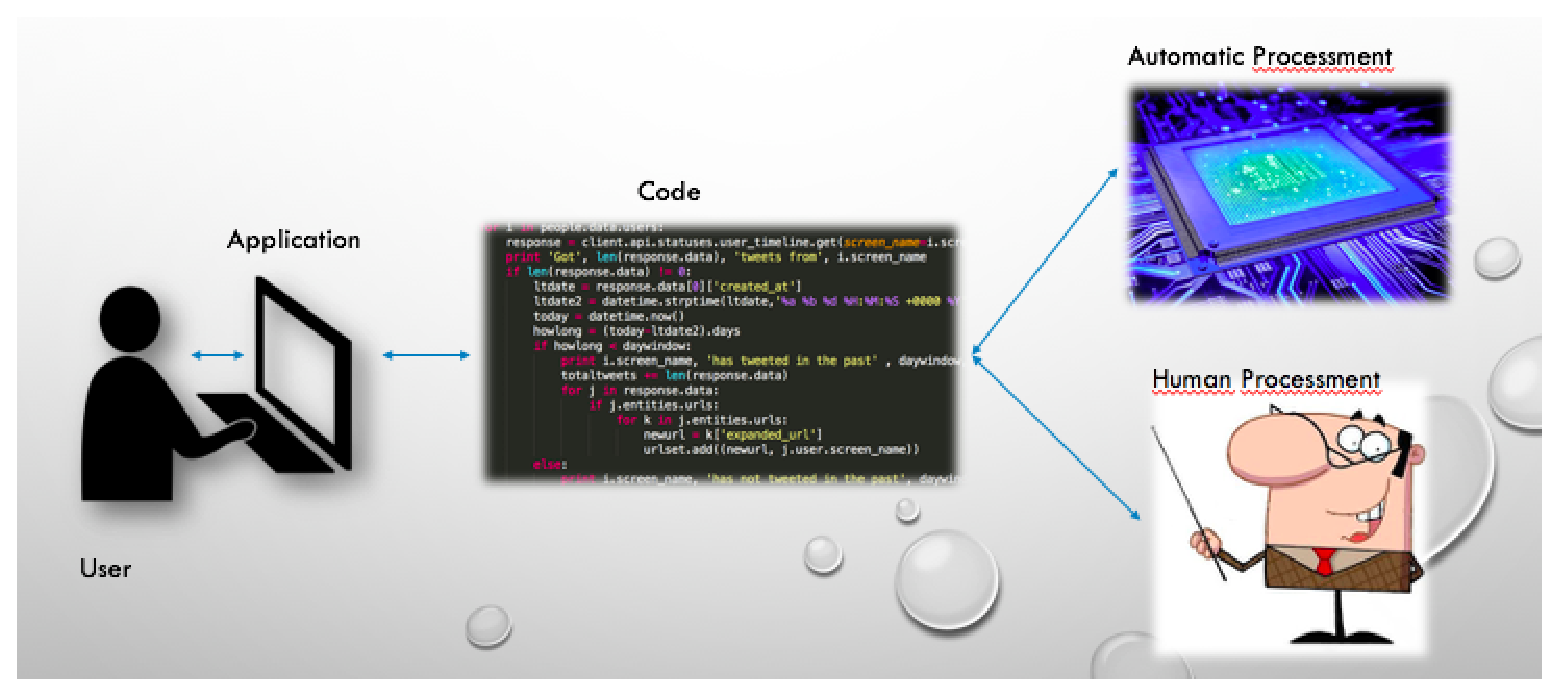
\includegraphics[scale=0.3]{figure/hc}
\caption{Human Computation}
\label{hc}
\end{figure}

Macrotasks require more effort from the worker, often requiring him to be an expert in the field or to have training on subjects related to the task. In the context of media annotation, this type of task is suitable for complex annotations because it assumes that the worker is qualified and will devote the time and effort required to complete it. However, macrotasks often require sophisticated annotation systems and limit the group of workers who are able to execute them \citep{Haas:2015:AMC:2824032.2824062}. In this work, complex annotations are defined as those that combine annotations on different aspects of annotated objects and therefore are usually obtained by macrotasks.

On the other hand, microtasks are usually modeled in a way that can be accomplished quickly and easily by less skilled workers. For media annotation, this kind of task is usually used to generate simple annotations, which refer to one or a few items to be annotated in each task. Also, often a Microtask can be performed using a simple annotation tool. 

Microtasks are widely used in crowdsourcing projects and this kind of task is supported by well-established commercial platforms such as Amazon Mechanical Turk, CrowdFlower and Microworkers.  According to these requirements microtasks should be:
\begin{itemize}
	\item{\textbf{Small:}} a worker must complete a task by means of few interactions, preferably by a single interaction.
	
	\item{\textbf{Quick:}} it should be possible to complete a task in a very short time, preferably within a few minutes.

	\item{\textbf{Easy:}} the easier the task, the less skilled the workers should be. Preferably, a task must be modeled so that it can be performed by any worker, just read the instructions and have the technical requirements for the task, such as minimal screen resolution, audio devices, or minimal Internet connection speed.
\end{itemize}


%In summary, annotated macrotasks often require more skilled workers and more sophisticated annotation tools, although they may result in more complex artifacts that represent more aspects about annotated media objects. On the other hand, microtasks can usually be performed by unskilled workers using simple annotation tools.

Moreover, considering each microtask as a human computing function, mapping elements from input to output, it is possible to understand that it is possible to compose an algorithm using these functions to obtain equivalent results generated by macrotasks \cite{Chen:2017:RIM:3025453.3025969}.



%Considering the pros and cons of both task classes, CrowdNote proposes a different approach to performing complex media analyzes.

%The division of a macrotask into a set of microtasks is something that is already done in some works \citep{Cheng:2015:BDC:2702123.2702146}, but CrowdNote presents a systematic way of doing so, making available guidelines and resources such as templates for simple annotation tasks and complex annotation production workflows. Moreover it is available CrowdNote Framework composed by process manager, a microtask manager and a library of simple annotation tools and aggregation methods.

%	\subsection{Microtasks}
%	In order to achieve complex media annotation CrowdNote uses a process workflow composed by a set of simple media annotation tasks. Each simple media annotation task is modeled as a microtask, following some requirements to make the process compatible with an unspecialized crowd and simple annotation tools. 

Microtasks are widely used in crowdsourcing projects and this kind of task is supported by well-established commercial platforms such as Amazon Mechanical Turk, CrowdFlower and Microworks.  According to these requirements microtasks should be:
\begin{itemize}
	\item{Small:} a worker must complete a task by means of few interactions, preferably by a single interaction.
	
	\item{Quick:} it should be possible to complete a task in a very short time, preferably within a few minutes.

	\item{Easy:} the easier the task, the less skilled the workers should be. Preferably, a task must be modeled so that it can be performed by any worker, just read the instructions and have the technical requirements for the task, such as minimal screen resolution, audio devices, or minimal Internet connection speed.
\end{itemize}

\pagebreak
In CrowdNote each microtask is modeled as a process composed by two steps: collection and aggregation. The collection step uses annotation tools to gather contributions from the crowd, and the aggregation step processes the collected data in order to generate the output. Actually, the updated version of CrowdNote supports both multiple outputs per microtask and three classes of aggregation methods.

Multiply outputs per task allow product at the same task different artifacts. It is possible at the same time generate a partial output to be used to feed the next task in the production workflow, even it is possible to generate an simple outcome such as datasets, sumaries, tag lists and more. The three classes of aggregation method are: automatic, manual and supervised.
 
\begin{itemize}

 
\item{Automatic methods} are rule-based and uses automatic filters, statistic techniques and convergence metrics to merge the contributions into an output.
 
\item{Manual methods} are used when is not possible to explicit a set of rules to generate the desired output. This kind of aggregation allows to use human intelligence to generate results which is very interesting in cases at the contributions involve emotions, subjectivity or creativity. 

\item{Supervised methods} are based on automatic method, although they combine human work to validate or adjust the aggregated result.
\end{itemize} 


In addition, simple media annotation tasks that follow CrowdNote requirements can be accomplished by very simple annotation tools, which can usually be simple Web forms. The CrowdNote Framework provides a library of aggregation methods and simple media annotation tools that can be used to create new projects, extended, even used as templates.


	\subsection{Crowdsourcing}
	%Human computation approaches can improve performance by the division of labor because it helps to execute tasks in parallel. Each worker performs their work independently so that the instances of a task can be executed in parallel, according to the Human Computation paradigm \cite{Rohwer:2010:NHC:1837885.1837897}.

To support the human computation paradigm, crowdsourcing has emerged as a proposal to annotate media objects using a large number of contributors efficiently \cite{VonAhn:2005:HC:1168246}. 
%Following the crowdsourcing principles, the tasks distributed to the workers are modeled to be done independently, maximizing the parallelism \citep{Howe2006}. Furthermore, each task can be sent to many contributors, allowing to compare, check and to aggregate the contributions, also reducing the chance of producing a biased result  \cite{GALTON1907}.

This approach generally delivers good quality results using contributions from the crowd and can distribute, collect, validate and combine large amounts of tasks results \cite{Mo:2013:OPH:2505515.2505755}. Since this approach is designed to handle a huge number of cooperators and contributions for tasks that require human intelligence \cite{Howe2006}, Crowdsourcing is appropriate to allow the Human Computing paradigm to be applied in a massive-scale online cooperation \cite{TEDMassive}. Crowdsourcing  is supported by four pillars:  The Crowdsourced Task, The Crowdsourcer, The Crowd, and The Crowdsourcing Plataform \cite{6861072}.

\begin{itemize}

\item{\textbf{The Crowdsourced Task}} is the HIT designed, according to the Human Computing paradigm, to acquire workers' contributions. Task instances are presented to the workers as jobs that must be performed \cite{Difallah:2015:DMC:2736277.2741685}.

\item{\textbf{The Crowdsourcer}} is the owner of a project, it may be an individual or institution that wishes to have a completed task. The owner is responsible for starting the crowdsourcing process, defining what task must be completed and how it should be presented to the workers as jobs \cite{6861072}.

\item{\textbf{The Crowd}} is the workforce that moves the process once it is composed of all the workers who perform the jobs needed to generate the outcome. Each worker carries out his work independently so that the works can be executed in parallel, according to the paradigm of Human Computation \cite{Rohwer:2010:NHC:1837885.1837897}.

\item{\textbf{The Crowdsourcing Platform}} is a computational system responsible to manage the whole process, serves as an entry point for both the owner making the tasks available and for the workers to execute them. This kind of environment can be something sophisticated such as CrowdFlower, Microworkers, and AmazonMechanical Turk \cite{Difallah:2015:DMC:2736277.2741685}, or really simple systems with screens and forms for data collection such as the mobile application used by the Google Crowdsource project \cite{google_cs}. A crowdsourcing environment is necessary, as the tasks must be made available to a potentially large number of workers. The crowdsourcing platform is a key element of support to massive-scale cooperation.

\end{itemize}

The use of a commercial crowdsourcing platform brings benefits such as not having to worry about management's issues of workers, jobs, and contributions such as employee recruitment and collection of contributions as well as facilitating employee payments. Also, payouts are a good way to motivate and keep the crowd, although there are other coping factors such as personal accomplishment and gamification.





	\subsection{The Wisdom of Crowds}
	Francis Galton wrote in 1907 an article in which he reported an experiment that a crowd of people at an agricultural fair tried to guess the weight of a particular ox. Galton verified that the average of the assumed weights converged to a value very close to the actual weight of the ox and analyzing the distribution of values grounded the Wisdom of the Crowd concept, according to which a heterogeneous crowd large enough tends to provide such a good expert result \cite{GALTON1907}. Additionally, James Surowiecki listed in his book "The Wisdom of the Crowds" \cite{surowiecki2005wisdom} four requirements for a crowd to deliver good results.

\begin{itemize}
\item{\textbf{Diversity:}} each person adds private information or bias.
\item{\textbf{Independence:}} people form their opinions independently.
\item{\textbf{Decentralization:}} people draw on their own knowledge.
\item{\textbf{Aggregation:}} a mechanism exists to turn private judgments into a collective decision.
\end{itemize}

Crowdsourcing platforms are environments suited to this theory, especially because it is possible to reach workers from different parts of the world and contexts with different backgrounds, which favors diversity. A common scenario in these environments involves workers receiving tasks and executing them without interacting with others, which helps create conditions for Independence and Decentralization.

For each task class, an appropriate aggregation method must be applied. These methods may involve convergence of responses, geometric means, contribution merging, as well as other types of processing. In this work, three categories of aggregation methods are also considered: automatic, supervised and manual.

\begin{itemize}

\item{\textbf{Automatic:}} an automatic aggregation method employs  algorithms to process the contributions in order to generate the desired outcome. This kind of method involves convergence analysis, geometric mean, instance prevalence and ranking. 

\item{\textbf{Supervised:}} in some cases its possible to apply automatic convergence methods, although is required additional human verification or some human interaction in the contributions' processing. 

\item{\textbf{Manual:}} manual aggregation is used when its not possible to define the rules or algorithm that should be followed to generate the outcome. These situations are usually related to subjectivity and emotional aspects that must be analyzed in the contributions to generate the result.

\end{itemize}

	
\section{Related Work}
	Crowdsourcing media annotation approaches are used in various applications and are used to gather information of various types, such as temporal synchronization\cite{wu2014crowdsourced}, events\cite{Kim:2014:JSL:2679600.2680027}, scene objects\cite{vidwiki2014}, emotions\cite{biel2013youtube}, actions\cite{riek2011guess}, and geo-tagging\cite{gottlieb2012pushing}. Among these works, \cite{Kim:2014:JSL:2679600.2680027,riek2011guess,wu2014crowdsourced} used microtasking approaches and unskilled workers, while \cite{vidwiki2014,biel2013youtube,gottlieb2012pushing} required skilled or trained workers to perform more complex tasks.

The work conducted by Kim \cite{Kim:2014:JSL:2679600.2680027}, he used a crowd to jointly summarizing large sets of Flickr\footnote{https://www.flickr.com} images and YouTube\footnote{https://youtube.com} videos in order to create novel structural summaries of online images as storyline graphs. The workers received a set of frames extracted from a video segment, and had to select some of them to create a summary. Once the set of convergent images were obtained, they were used to find similar images on a dataset extracted from Flickr.

Riek used a game approach \cite{riek2011guess} to annotate a video dataset with tags related to facial expressions, posture, gestures and more. The crowd used a very simple annotation tool in which they could insert tags by clicking buttons.

VidWiki\cite{vidwiki2014} is a complex system to improve video lesson by annotating them, which provides a complex annotation tool that allows the worker to edit video scenes by adding various types of annotations, including LaTex equations. This system requires some skills, including knowledge about Latex\footnote{https://www.latex-project.org}.

An important observation of the works related to crowdsourcing media annotation is that, in general, microtasks are performed by unskilled workers using simple annotation tools, to obtain simple annotations. On the other hand, jobs that aim at complex annotation often use larger tasks that require skilled or trained workers as well as more elaborate tools.

\section{CrowdNote}

\subsection{Method} 
	--	Full Paper Webmedia 2017 \cite{172450}

The crowdsourcing video annotation approach presented in this paper follows three steps: Preparation, Annotation, and Presentation. 

The preparation step describes how a complex annotation task can be divided into simple microtasks, in addition, is presented a workflow for the activities required before the annotation step, such as to define what should be annotated and the annotation types, as well as to design the microtasks and the simple annotation tools to execute them. In the annotation step, the annotation microtasks are performed by crowd workers, that are the contributors to the process. This step follows a workflow in which each microtask is followed by a specific aggregation method that generates a result so that the output from a task feeds the next one. The presentation step displays the outcome delivered by the annotation step, also at this point, all partial results are available to be used in other applications. The approach introduced also allows the development of expansive video annotation systems in which it is easily possible to add new microtasks to improve its result or generate new results. 

These steps contain specific activities and are executed sequentially how can be seen in Figure~\ref{process}.

\begin{figure}[h]
	\centerline{\includegraphics[scale=0.4] {figure/process}}
	\caption{Process workflow}
	\label{process}
\end{figure}

\textbf{Preparation:} all activities involved in this step are performed by the owner, who started the video annotation process. At this step is determined what must be annotated, also how they should be annotated. In this way the owner must determine:
\begin{enumerate}
\item What kinds of point of interest should be annotated.\\Ex: events, objects, subjects, issues.
\item What annotation type will be used for each of these kinds.\\Ex: free write, item selection, button click, image upload.
\item What data type will be collected for each annotation type.\\Ex: plain text, location, image, video.
\end{enumerate}

To illustrate this point, the example of the football(soccer) match annotation will be recalled. In a football(soccer) match video the kinds of point of interest correspond to events such as goals, cards, and faults. For each point of interest observed it should be collected its kind, and the instant when this event happened. The annotation type to be used on the annotation tool can be a set of icons related to each event. Finally, the data type collected in this case may be plain text that contains the kind of event identified and the instant it happened \cite{santos2007estrategia}.

Also, it is important to provide explanations or guidelines that can instruct the workers about how to execute the microtasks. An additional activity on the Preparation step is to determine what section of the video should be sent by each worker, this division can be made by duration (ex: send a 5 seconds segment to each worker), or using contextual criteria such as to send to each user a segment that contains a single dialog. The activities sequence for this step can be observed in Figure~\ref{preparation}.

\begin{figure}[h]
	\centerline{\includegraphics[scale=0.4] {figure/preparation}}
	\caption{Preparation step}
	\label{preparation}
\end{figure}


\textbf{Annotation:} An essential aspect of this step is to determine the microtasks' workflow, so the output from a task is taken as input by the next one, generating an outcome at the end of the last microtask. This cascade workflow is illustrated in Figure~\ref{cascading}. It is important to notice that each task cell in composed by two activities, the microtask in self and the aggregation method, that generates the output from the obtained contributions. In this way, the output from the last task cell is the outcome provided by the system.

\begin{figure}[h]
	\centerline{\includegraphics[scale=0.25] {figure/cascading}}
	\caption{Annotation step for N microtasks}
	\label{cascading}
\end{figure}

\textbf{Presentation:} at this step is generated an annotated video including the original video and the final outcome from the previous step. Other activities that can be proceeded at this step is to generate or to render, media items selected from the crowd annotations, as well as aggregate these items over the videos to compose a multimedia presentation.

\begin{figure}[h]
	\centerline{\includegraphics[scale=0.5] {figure/presentation}}
	\caption{Presentation step}
	\label{presentation}
\end{figure}










\subsection{Framework}
	Figure~\ref{architecture} shows the framework designed to support our method. This framework offers specific tools that help the design and aggregation of tasks, which are essential activities to put our proposed method in practice.

%\begin{figure*}[ht!]
%	\centerline{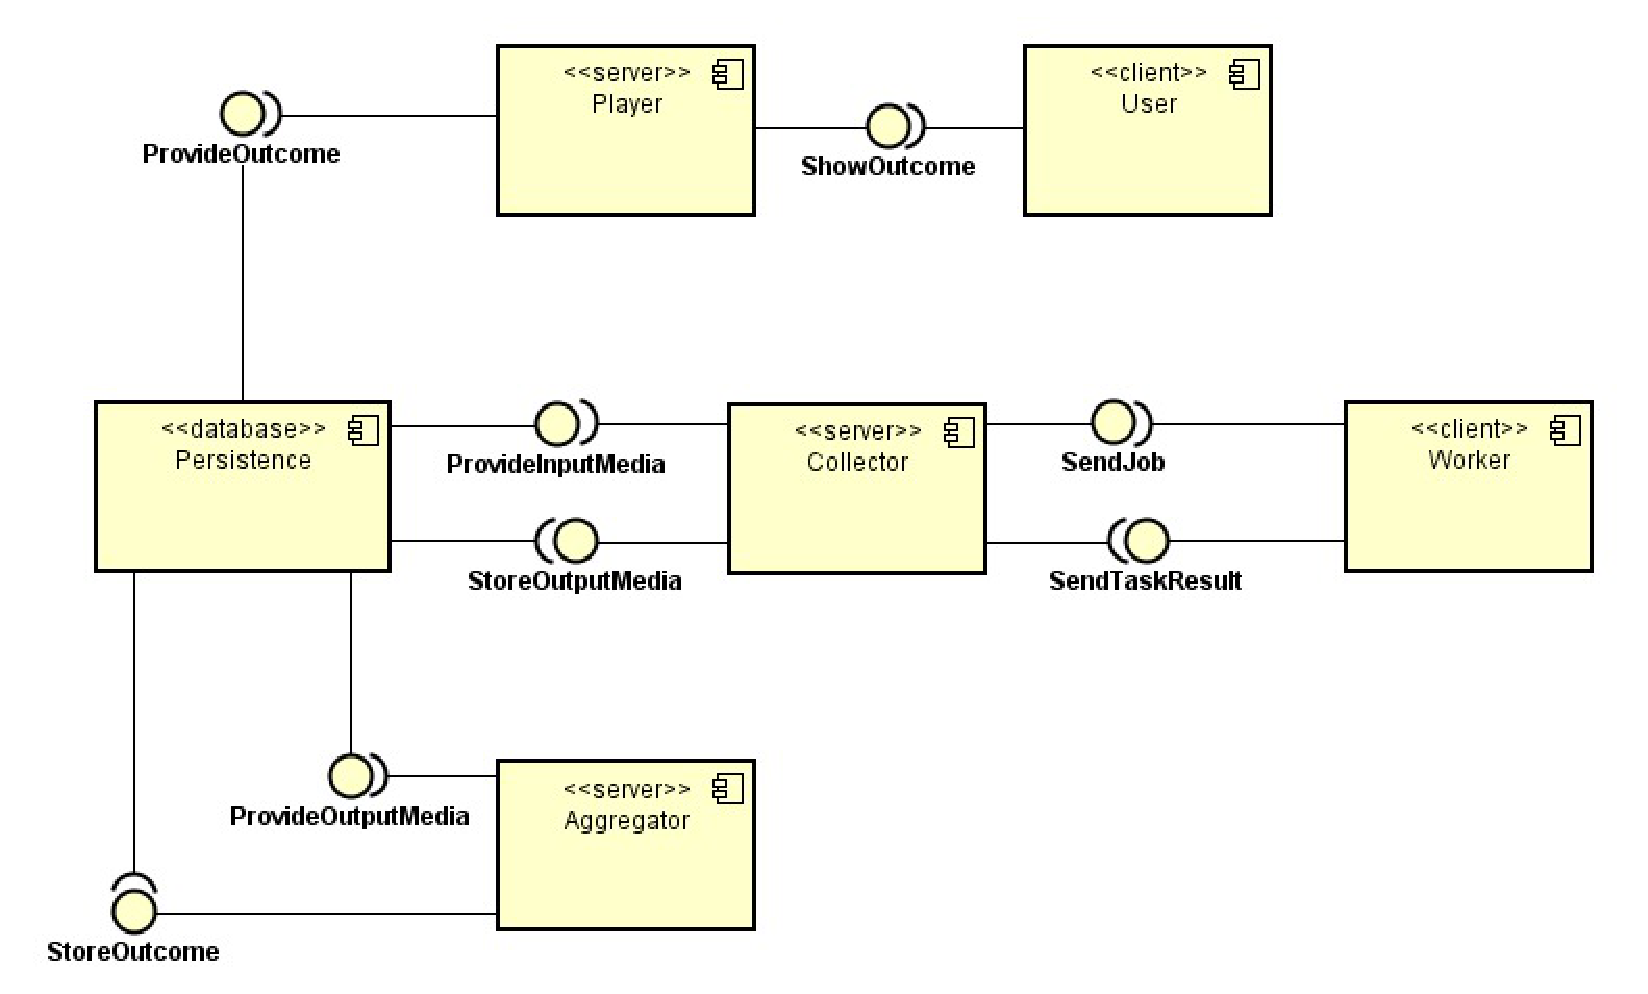
\includegraphics[scale=0.5] {figure/system}}
%	\caption{Framework Architecture}
%	\label{architecture}
%\end{figure*}

\subsection{Database}
%The database module contains the persistence component that is the point of communication between the modules of the structure. In this way, the modules can be decoupled, increasing the flexibility of the system and the possibilities of integration with external environments in a service-oriented architecture. 
%The communication interfaces between the persistence component and the others can be seen in Figure~\ref{persistence}.

%\begin{figure}[h!]
%	\centerline{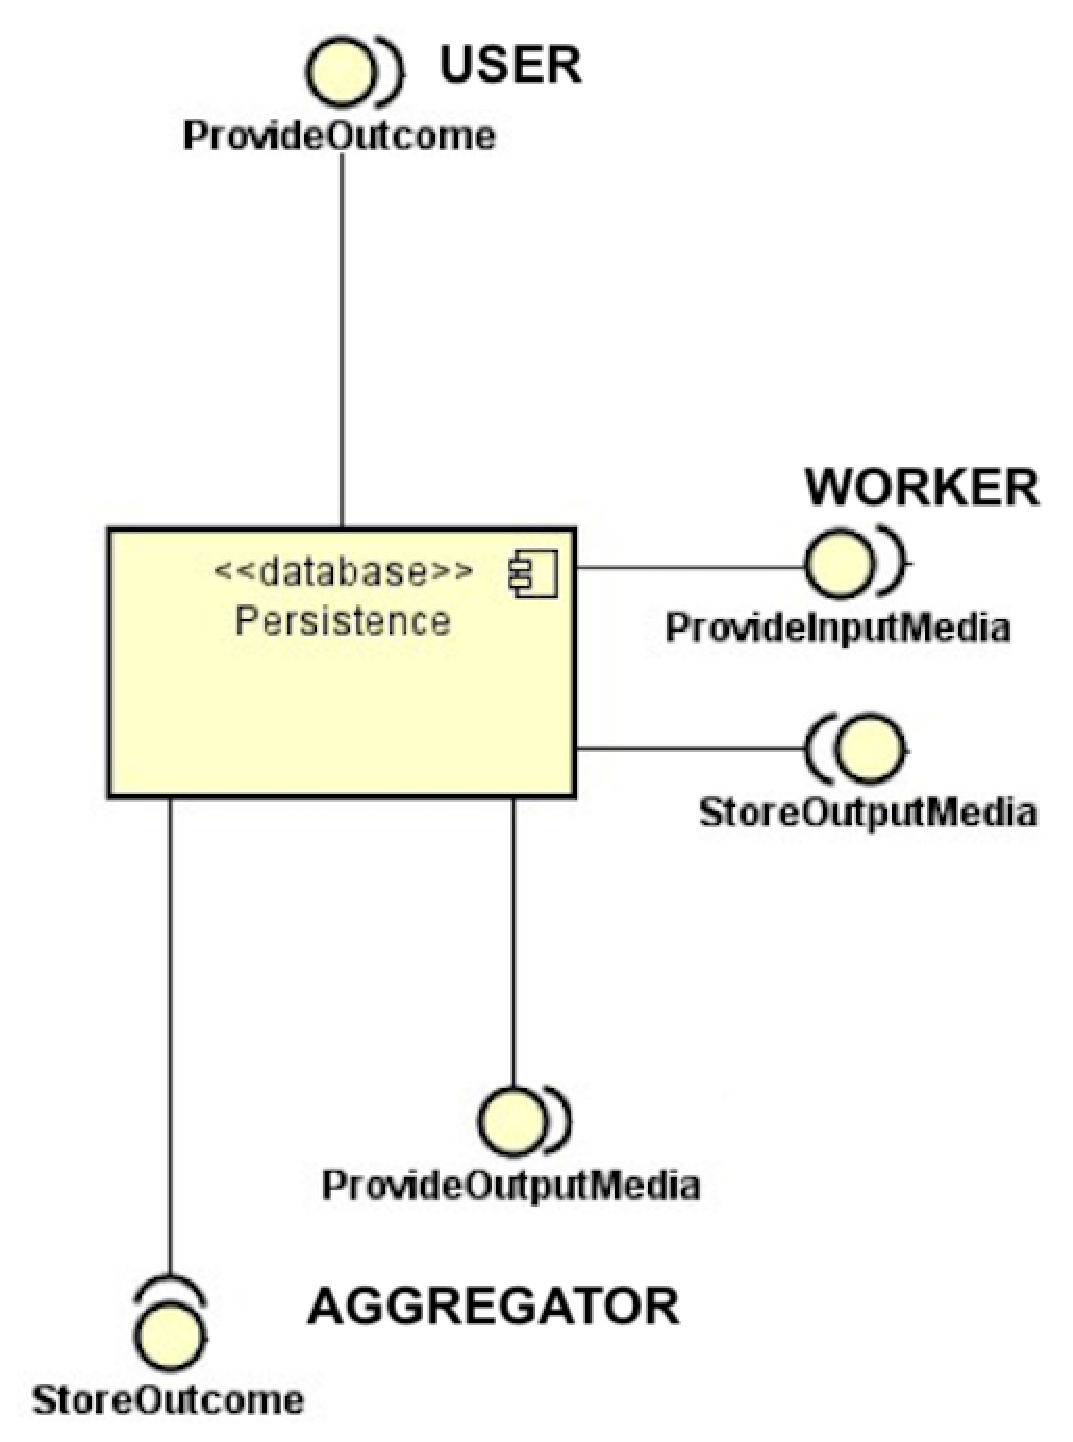
\includegraphics[scale=0.25] {figure/persistence}}
%	\caption{Persistence component}
%	\label{persistence}
%\end{figure}


The persistence component sends to the server module the information required to render in the client both, the job requests to workers and the content needed to present the result to the users. Once the persistence component communicates with its own database.
%, there is no need for the crowdsourcing platform, if used, to have access to the dataset.

Likewise, contributions provided by workers are sent directly from the collector to the persistence component, so that they are stored directly in the database without having to go through the external crowdsourcing environment in no time

The aggregation component also communicates directly with persistence. The aggregator requests each run the collected contributions to a task and, after the aggregation process, sends the result to be stored from the database to be used as input to the next task, again maintaining data privacy because it does not need to be stored in any external environment.

\subsection{Server}
The server module is responsible for distributing the jobs, managing contributions, and controlling the active task in order to execute the process workflow. This module is composed of three components: Collector, Aggregator, and Player. 

\begin{itemize}
\item \textbf{Collector: } The collector feeds an annotation tool with the information about the item to be annotated, so it renders the job's interface used by the worker to perform the task. Completely, this component is also responsible for gathering the information provided by the worker in the execution of the task and sends them to the persistence so that they are stored.

\item \textbf{Aggregator: }The aggregator verifies, filters, groups, and processes the collected annotations of the crowd according to the rules defined for each task. In this update version, the aggregation process can be fully automatic, supervised or manual. Manual aggregation is useful when is desired to evaluate each contribution as in authoring tasks. Supervise aggregation can be a good option when is possible to apply automatic methods but is required human verification of the result. Automatic aggregation is the default choice, this class of methods includes grouping, comparing, counting, calculating and other operations.

\item \textbf{Player: } The player component works in a  similar way to the collector, although it renders the content to users and its communication with the persistence is unidirectional. It feeds the client player tool with the metadata, the extra content, and the original video. Thus, the player tool on the client can play the enriched video synchronously.
\end{itemize}


\subsection{Client}
The client module manages the communication interfaces with workers and users. The approach used is to use templates that are fed with the descriptive data of the visualization to be generated.

In this way, it is possible to keep the entire control part on the server, accessible through the collector and player components, and therefore templates can be stored anywhere if it is accessible on the internet. This allows contributions to be collected from crowdsourcing platforms and web pages published on different hosts. In fact, this strategy allows to collect entries from different sources at the same time.

Both the container collection view and the final content view display work in a similar fashion. According to the desired visualization, a model is selected and the server module is queried to obtain the necessary data to render the desired interface. 

%This process is illustrated in Figure~\ref{rendering}.



%\begin{figure}[h!]
%	\centerline{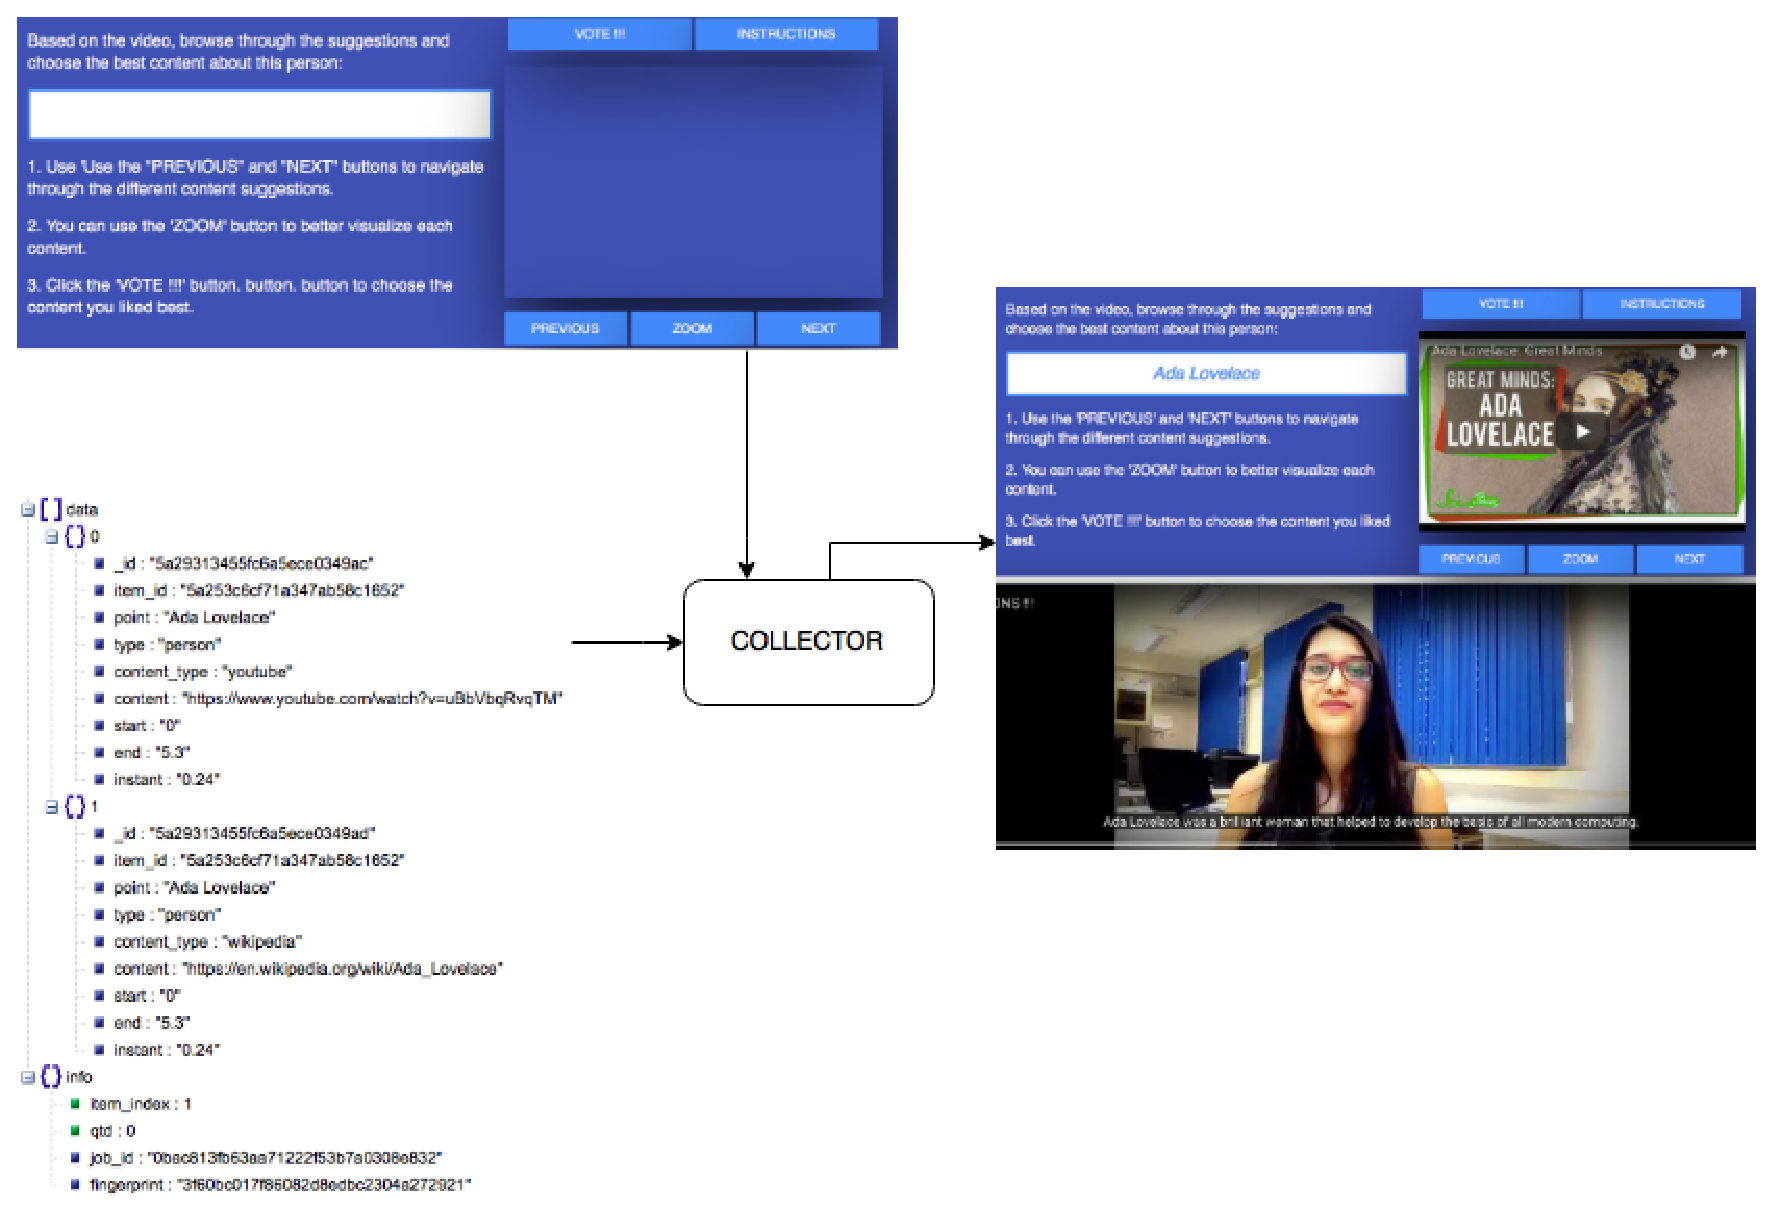
\includegraphics[scale=0.28] {figure/rendering}}
%	\caption{Job rendering}
%	\label{rendering}
%\end{figure}


The interaction between the system modules through the interfaces are described as follow:
\begin{itemize}
\item \textbf{Provide Media Input:} To generate each job to be sent to a worker, the Collector receives an entry from the Persistence component.

\item \textbf{Send Job:} The Collector sends a job to a Worker who sees the task through the Client and executes it.

\item \textbf{Send Job Result:} The Client sends to the Collector the annotation made by the Worker for the job received.

\item \textbf{Store Media Input:} The Collector sends the collected contribution to the Persistence that stores it in the Database.

\item \textbf{Provide Output Media:} The Persistence send to the Aggregator all the collected contributions for a task.

\item \textbf{Store Outcome:} The Aggregator stores the resulting entries from the aggregation process in the Input collection so that they are supplied as input to the next task.

\item \textbf{Provide Outcome:} The Aggregator sends the outcome to Persistence to store it.

\item \textbf{Show Outcome:} The Player displays to a User the outcome generated by the cascading microtasks process.

\end{itemize}

The next section describes how we used this framework to apply our method in a video enrichment case study.

















\section{Case Study}
	The experiment used the presented method to enrich videos with additional semantic information about characters, theories, and technologies mentioned. The rich video generated is a self-contained multimedia document, so the user doesn't need to use other sites or databases to access supplementary content for the points of interest.

Each supplemental content can be accessed through trigger items that are images and labels that appear in scenes where the point of interest is mentioned. When the trigger items are clicked, the video pauses the extra content is displayed so they can be viewed, and when closed, video playback resumes normally.

The crowdsourcing process used in the experiment followed a workflow of 4 annotation microtasks. Each of these simple tasks was modeled that could be performed by a worker through a simple tool annotation, only that the worker could understand the language spoken in the video. The video was produced in the English language and features an actress narrating a text about the history of computing.
\pagebreak
%Preparation and Annotation processes, including workflow construction, microtasks definitions, annotation tools, the aggregation methods, as well the results obtained in each microtask will be described below.

\subsection{Our Crowd}
To reach a heterogeneous crowd, the Microwokers \cite{microworkers} platform was used, this platform was used only to recruit and pay workers, and the whole process was supported by the developed system.

Microworkers proposes different models for a crowdsourcing process. Initially, you can choose between starting a basic campaign or using contracted groups.

In a basic campaign, all registered workers in the system can see the task on the job wall and accept to run it. A campaign that uses hired groups allows you to select the crowd by choosing groups of workers with a certain profile. In addition, it is possible to create lists with good workers who have made good contributions to recruit them for other tasks. Some of hired groups available in Microworks are listed in Figure~\ref{groups}.
\begin{figure}[h!]
 \centerline{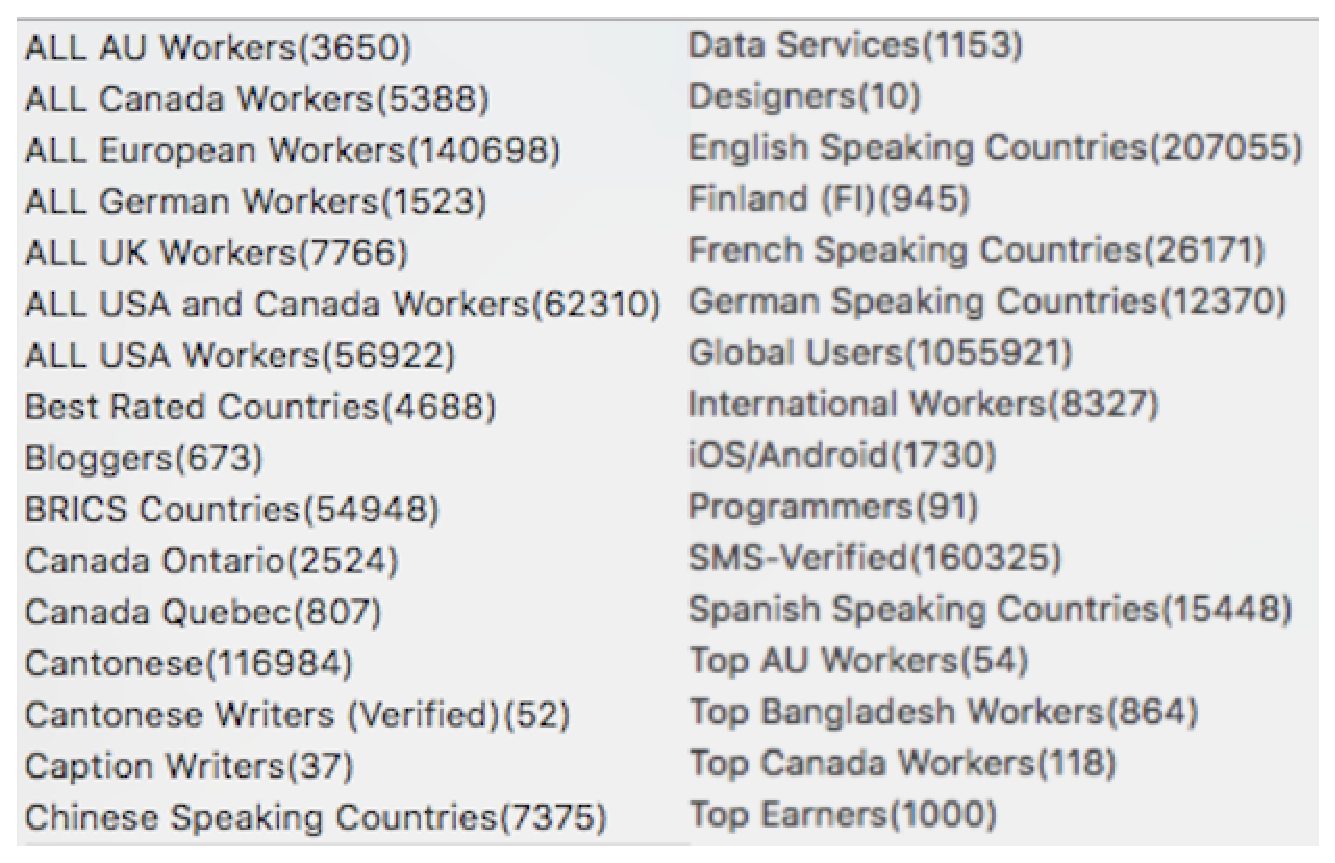
\includegraphics[scale=0.25] {figure/groups}}
	\caption{Microworkers Hired Groups}
	\label{groups}
\end{figure}

The purpose of this paper is to use unskilled workers, although it was necessary for them to know enough of the English language to understand the video used in the experiment. In this way, the tasks were launched as campaigns that used contracted groups, to increase the chance of the workers who contributed in a task also to participate in others, was chosen a group of moderate size and with workers relatively assiduous so that the contributions were made more quickly. The group chosen was Data Services, with 1153 potential workers to accept the jobs.

Some groups are made up of workers who only accept tasks that offer slightly larger payments, but considering the group chosen, it was feasible to offer a payment of 2 cents per task. Also, each task was active for 24 hours to reach all time zones in the same way.

\subsection{Preparation}

The preparation step began with the identification of the micro-tasks needed to achieve the expected result. Since the goal was to generate enriched videos through supplementary content at points of interest, it was determined that they were needed. Thus, it was determined that 4 microtasks would be performed:

\begin{itemize}
\item Identify the points of interest in the video; 
\item Gather content suggestions for each point of interest; 
\item Determine the most accepted supplementary content for each point of interest; 
\item Position the trigger items at the best position over the video. 
\end{itemize}

In relation to the distribution of the items to be annotated in each of the tasks, a circular list policy was adopted. In this way, there was a greater chance of each task, each item being annotated received the same number of contributions.

It was also necessary to determine how the video should be segmented to generate the input of the first task. The strategy chosen was to target the video based on the automatic captions generated by youtube. In this way, it was possible to generate short segments, but they tend to contain complete sentences. This method divided the video into 13 segments.

For budget and time issues, it was determined that the minimum amount of contributions each item could receive was 5, so Task 0 should receive at least 75 contributions. The number 5 was chosen because it is odd, which avoids drawings, and because it is an amount that already allows seeing a tendency of convergence of opinion in a heterogeneous multitude.

\subsection{Annotation}
In this section will be described the 4 annotation tasks, as well the annotation tools, aggregation methods and results for each of them. Because there is a dependency order between these tasks, it's not possible run them in parallel. In this way, an execution workflow in which the output of one task is used for the next one, as can be seen in Figure \ref{workflow}, in which the tasks are identified as T0 to T3 and their respective aggregation activities as AG0 to AG 3. The payment activities are identified as IA0 to IA3.

\begin{figure}[h]
	\centerline{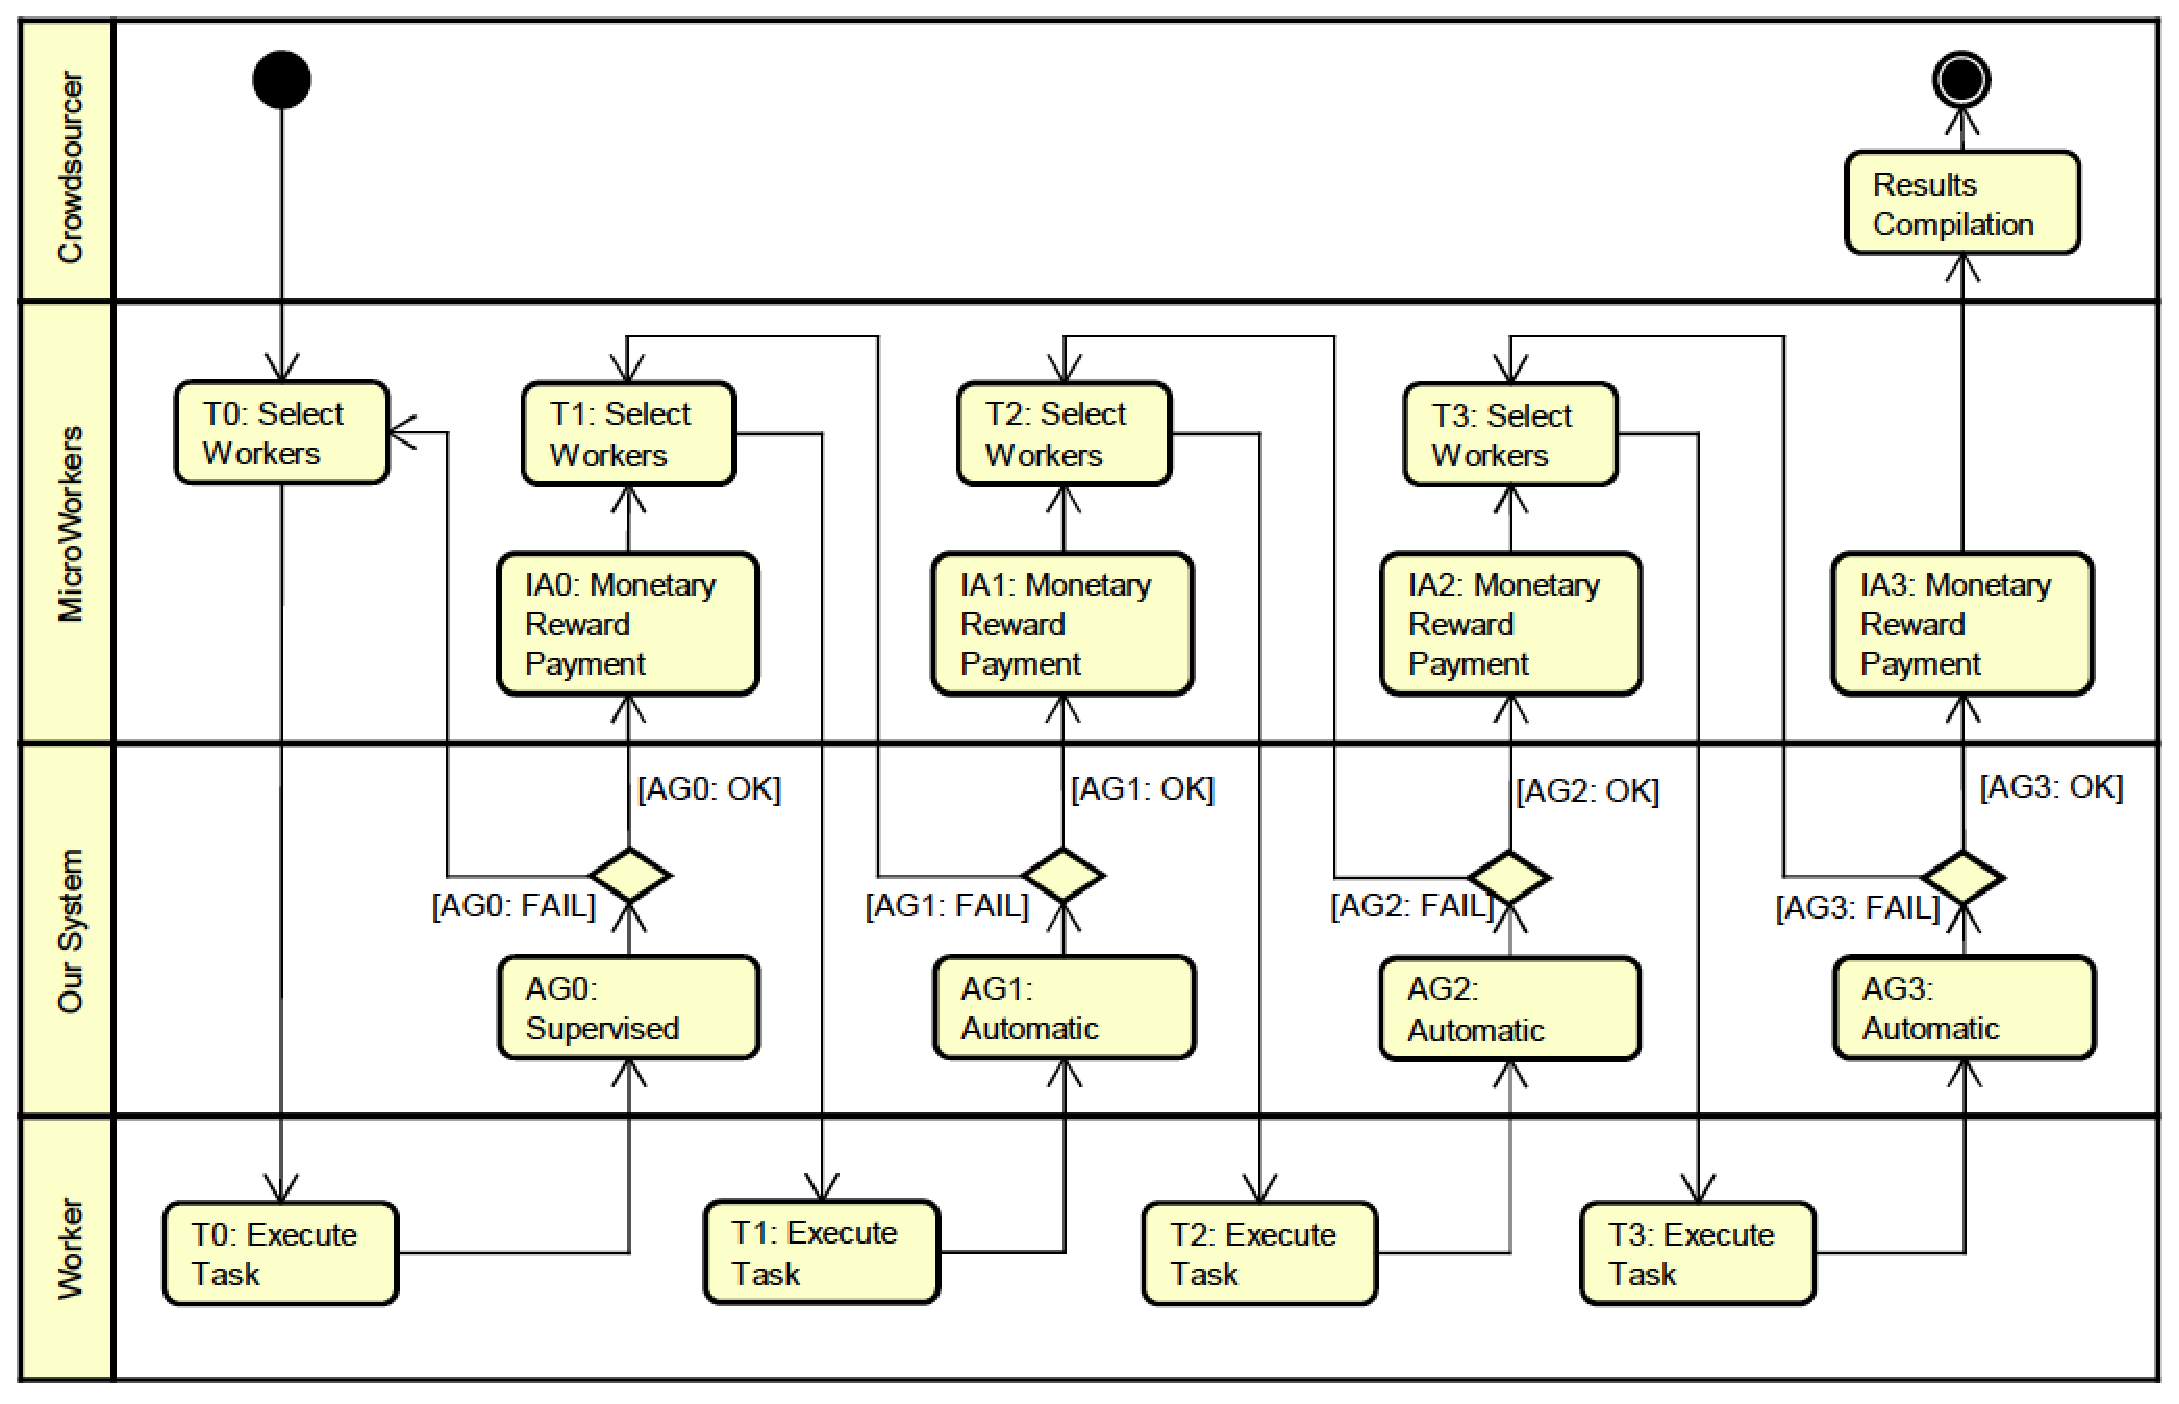
\includegraphics[scale=0.235] {figure/case}}
	\caption{Video Enrichment Workflow}
	\label{workflow}
\end{figure}

%Each of the four tasks applied to the workers will be described below, as well presented the annotation tool used for them.

\subsubsection{Task 0}
%\textbf{Identify Points of Interest:} The first annotation microtask is supported by the tool represented in Figure~\ref{task_1}, collecting identification for points of interest. In this task, the contributor receives a segment of video that should be watched, and if was found any point of interest, it should be marked and briefly described. These points of interest can be gestures, words, expressions, facts, concept, characters, events or anything that can be related to extra content.


\begin{itemize}
\item \textbf{Title:} Identify Points of Interest.

\item \textbf{Description:} A video segment is displayed to the worker and he must identify the moment at which a point of interest appears or is mentioned. This point of interest can be a person, a technology or a theory.

\item \textbf{Objective:} Identify points of interest in a video segment.


\item \textbf{Input:} A dataset with 13 video segments of 4.5 to 7 sec.


\item \textbf{Output:} A set of points of interest and the instant when they happen. In addition to serving as input to Task 1, this result also generated a summary based on points of interest.


\item \textbf{Instructions:} \begin{enumerate}
	\item Identify in the video something that you found interesting.
	\item Pause the video the moment it appears.
	\item Select its type: Person, Technology or Theory.
	\item Write what you have identified. 
\end{enumerate}

\item \textbf{Annotation Tool:} The tool is represented in Figure~\ref{task_0}.
\begin{figure}[h!]
	\centerline{\includegraphics[scale=0.17] {figure/task_0}}
	\caption{Annotation Tool for Task 0}
	\label{task_0}
\end{figure}

\item \textbf{Aggregation:} For this task, a supervised aggregation method was chosen in which the human interaction occurs at the end of the process. The contributions are filtered discarding the useless contributions (empty, nonsense, bad works), and the valid contributions are candidates to Points of Interest. The candidates are grouped in 2-seconds interval ranges. In each group, a similarity analysis is done and the most frequent occurrence is selected. Finally, the human supervisor edits the selected label so that the text is visually pleasing. The aggregation method extracted 11 Points of Interest from the 75 contributions.

\end{itemize}



\subsubsection{Task 1}

%\textbf{Provide extra content suggestions:} The second task took as input the aggregated result from the task 1 that is a list of points of interest identified by the workers. This microtask is supported by the annotation tool represented in Figure~\ref{task_2}. This tool presents to the worker a point of interest and the video segment positioned at the moment it occurs. This way, is possible to use the video for reference and contextualization.



%Through this tool, the worker can contribute by writing a text related to the point of interest, sending an image or sending a link to a YouTube video or a Wikipedia page.


%When the collection of contributions for this task is done, the Aggregator groups the content of the sender by a point of interest, and then joins the similar suggestions. In this way, a list of points of interest with a set of content suggestions for each is added to the next task, without repeated suggestions.

\begin{itemize}

\item \textbf{Title:} Provide Suggestions for Extra Content.

\item \textbf{Description:} In this task, the worker receives a point of interest and the video synchronized at the moment it occurs. The worker should suggest extra content to complement the video, which may be a short text, an image or a link to a YouTube video or a Wikipedia page.

\item \textbf{Objective:} Obtain from the crowd extra content to each point of interest.


\item \textbf{Input:} The set of points of interest collected in Task 0.


\item \textbf{Output:} A set of extra content associated with each point of interest. Each extra content may be an explanatory text, an image, even a link to a Wikipedia page or a Youtube video. Besides feed the Task 2,this output is also used to generate a content-based index to the video.


\item \textbf{Instructions:} \begin{enumerate}
	\item Select the type of content to send.
	\item You can upload an image, write a short text.
	\item You also can paste a link to Youtube or Wikipedia.
\end{enumerate}

\item \textbf{Annotation Tool:} The tool is represented in Figure~\ref{task_1}.
\begin{figure}[h!]
	\centerline{\includegraphics[scale=0.165] {figure/task_1}}
	\caption{Annotation Tool for Task 1}
	\label{task_1}
\end{figure}

\item \textbf{Aggregation:} For this task was chosen an automatic aggregation method. The filtering step discarded the corrupted files and broken links. The suggested contents were grouped by point of interest, and the duplicated items were merged. The aggregation method extracted 34 different suggestions of extra content from the 55 contributions received. All 11 points of interest received at least 2 content suggestions, some of which received 4 or 5. 
%The ideal case would be to obtain a more even distribution, although the result obtained was enough to continue the process.

\end{itemize}



\subsubsection{Task 2}



\begin{itemize}

\item \textbf{Title:} Ranking Suggestions.

\item \textbf{Description:} The worker receives a point of interest and the video positioned at the moment it occurs. It also gets the list of suggested extra content to complement this point of interest. The job is to choose the extra content that best complements the content related to the point of interest.

\item \textbf{Objective:} Determine the best extra content to each point of interest, according to the crowd.


\item \textbf{Input:} A set of points of interest, with the suggested contents associated with each one.


\item \textbf{Output:} An updated set of points of interest with the extra contented associated with each one. This output also can be used to generate a ranked list of alternative extra contents to supplement the points of interest.


\item \textbf{Instructions:} \begin{enumerate}
	\item Use the buttons bar to navigate through the contents.
	\item You can use the zoom button to visualize each content.
	\item Vote for the content you liked best.
\end{enumerate}


\item \textbf{Annotation Tool:} The tool is represented in Figure~\ref{task_2}. This tool has a drag-and-drop feature that lets you drag the item through the video until you find the appropriate position.
\begin{figure}[h!]
	\centerline{\includegraphics[scale=0.165] {figure/task_2}}
	\caption{Annotation Tool for Task 2}
	\label{task_2}
\end{figure}

\item \textbf{Aggregation:} This simple automatic aggregation method determines the most popular extra content suggested to each point of interest. As the contents were associated with 11 points of interest, were collected 55 contributions. In the filtering step the suggestions without votes was discarded. Finally, was generated an output with all 11 points of interest and the extra content associated with each one. 

\end{itemize}



\subsubsection{Task 3}

\begin{itemize}

\item \textbf{Title:} Determine the Position of the Trigger Items.

\item \textbf{Description:} This task consists of placing a trigger item in a video scene. This trigger item is represented as a rectangle containing a text or an image and should be positioned so as to minimize occlusions of important scene objects.

\item \textbf{Objective:} Determine the best position to display each trigger item over the video.


\item \textbf{Input:} A set of points of interest with the extra content associated with each one of them.

\item \textbf{Output:} Aset of points of interest with the extra content associated with each one, including now the position where each item should be displayed over the video. These positions are represented as coordinates (X,Y). The output of this task is the outcome of the video enrichment process, and can be executed in the Player. In addition, the metadata can be used to generate alternative outputs such as NCL to reproduce them in digital TV environments.


\item \textbf{Instructions:} \begin{enumerate}
	\item Drag the item by the video until finding the best position.
	\item When you have decided on the best position, click send.
\end{enumerate}


\item \textbf{Annotation Tool:} The tool is represented in Figure~\ref{task_3}.
\begin{figure}[h!]
	\centerline{\includegraphics[scale=0.17] {figure/task_3}}
	\caption{Annotation Tool for Task 3}
	\label{task_3}
\end{figure}

\item \textbf{Aggregation:} The automatic aggregation method applied at the final of this task determines the position at each item should be displayed over the video. The contributions for each item were grouped and the very discrepant positions of the others were discarded. Then, for each item, the average geographic position was calculated based on the X and Y coordinates predicted in the contributions. Was collected 55 contributions, of which 38 were after filtering. Of these 38 contributions were extracted the positions of the 11 items related to the points of intersection.

\end{itemize}


\subsection{Presentation}

The presentation system, shown in Figure~\ref{player}, receives the video, extra content, and necessary metadata from the Player Provider. This system is capable of reproducing the original video synchronized with the extra content, that is displayed every time a point of interest happens in the video. Is important to remind that all extra content displayed with the video was provided, selected and positioned by the crowd.



\begin{figure}[h!]
	\centerline{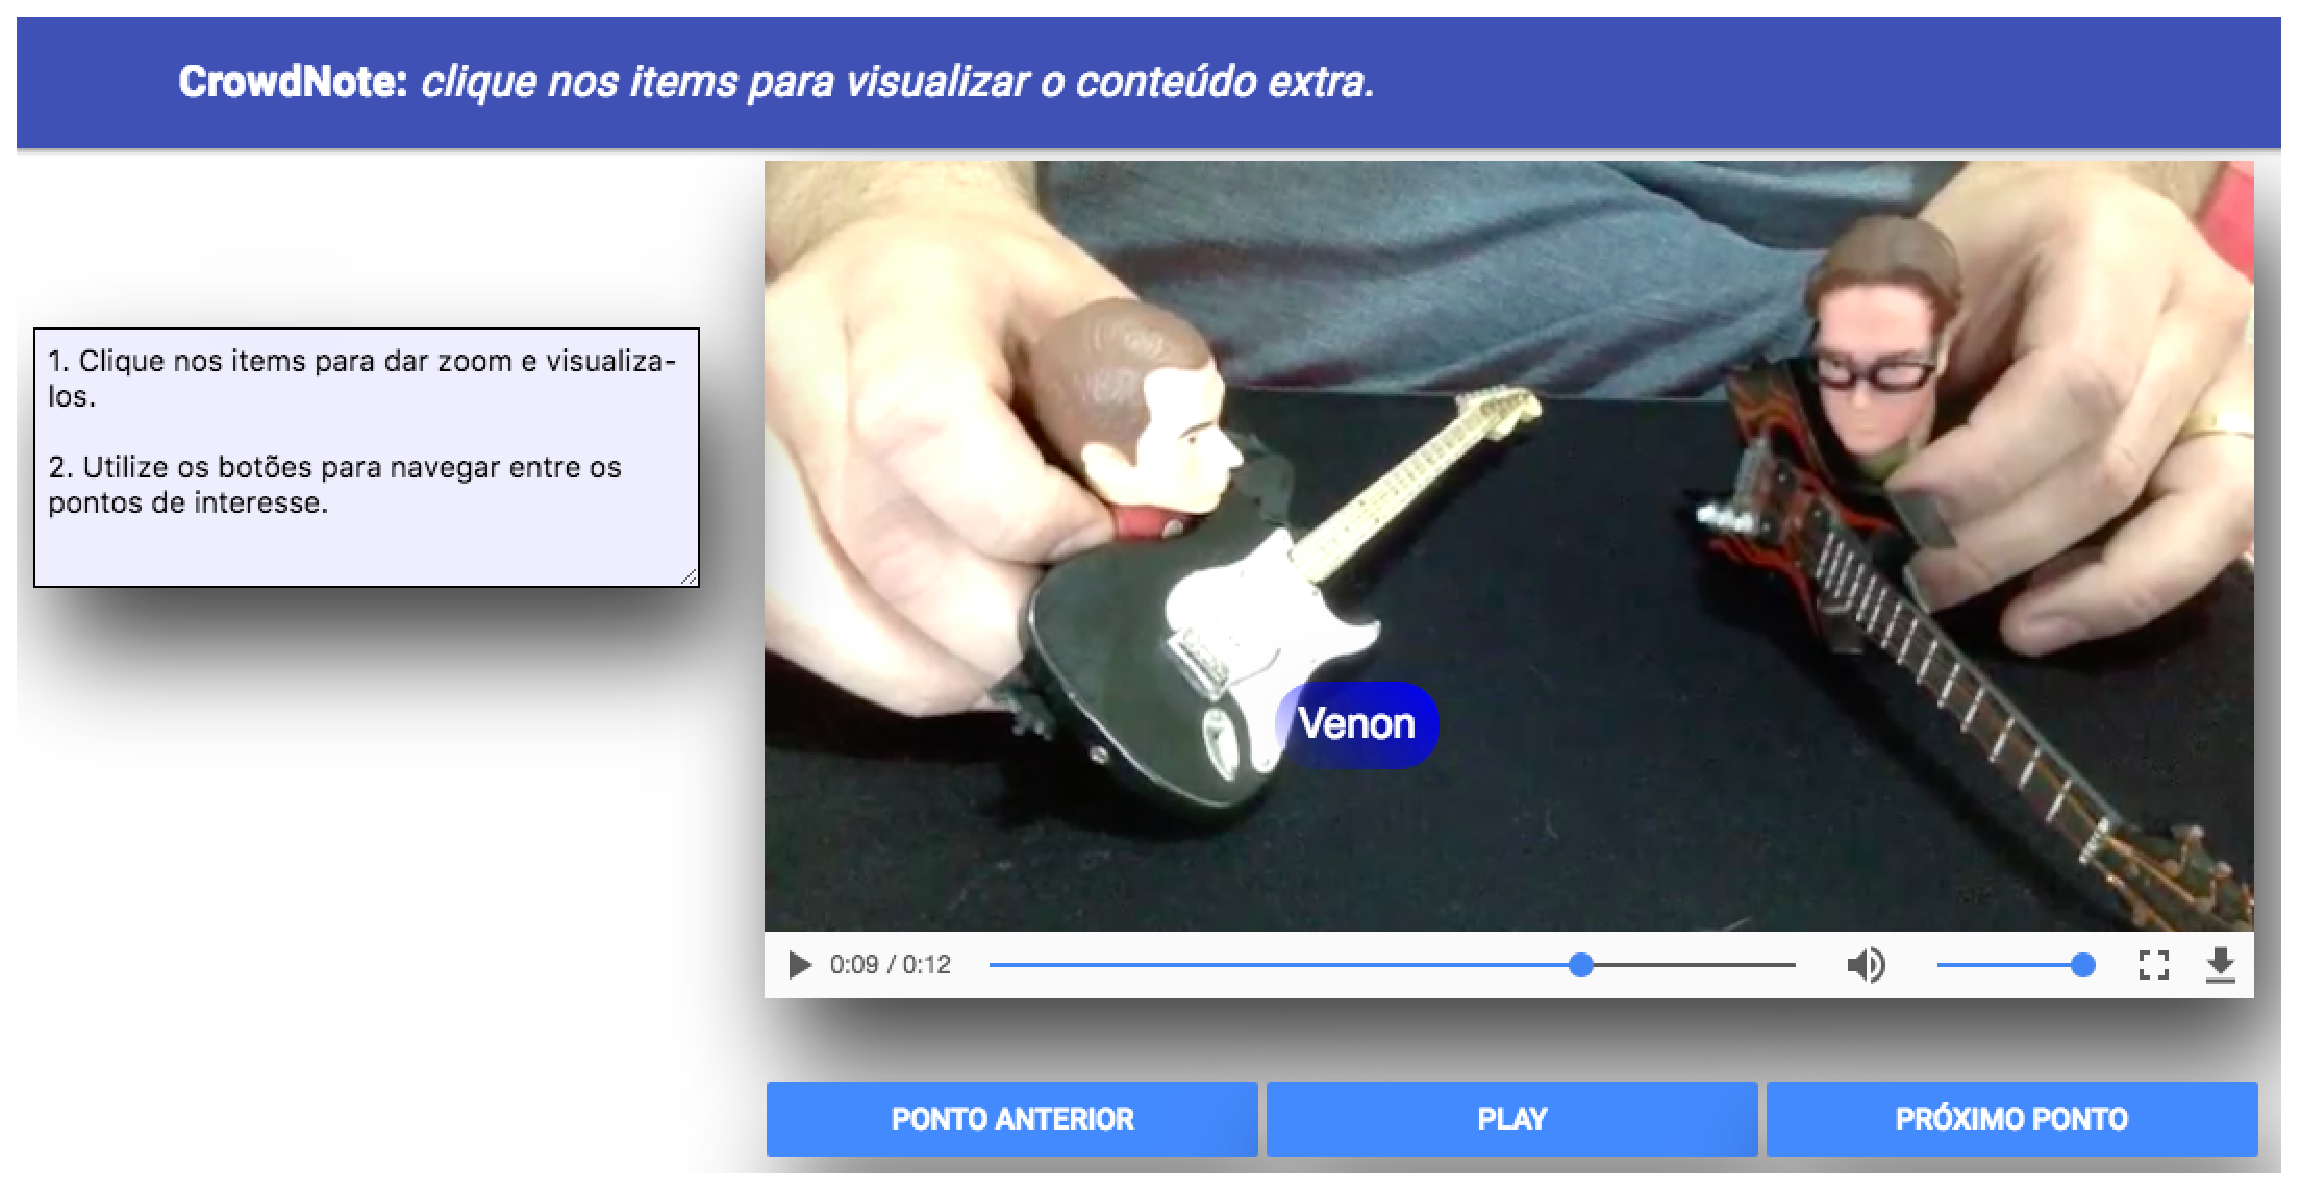
\includegraphics[scale=0.17] {figure/player}}
	\caption{Displaying an extra content item over the video}
	\label{player}
\end{figure}

This tool has a control bar with 3 buttons: Previous, Next and Zoom. These buttons are used to control two useful features, the content zoom and the navigation by point of interest.

The navigation by point of interest uses the list of points as a content index, allowing the user to navigate between points of interest by clicking the Previous and Next buttons. The Player automatically syncs the video at the time the current point of interest occurs.

When the user clicks the trigger item or the Zoom button, the extra content associated with the current point of interest is displayed on an upper layer as the video is paused. When you close the extra content, the video resumes its execution from where it was. The zoom view can be seen in Figure~\ref{player_zoom}.

\begin{figure}[h!]
	\centerline{\includegraphics[scale=0.17] {figure/player_zoom}}
	\caption{Player Zoom}
	\label{player_zoom}
\end{figure}



 \subsection{Runtime Observations}
 
During some tasks were observed some interesting facts about the behavior of workers. Keeping in mind that the motivation of the workers in the experiment was the payment and that the amount paid for each job was small, the workers tended to do the bare minimum. This aspect proved to be correct that the decision was made to use microtasks that needed only a simple interaction to be completed.
 
The reflection of this led to some decisions during the experiment, as in Task 1. In this task, the worker was asked to suggest extra content to supplement the points of interest and for this, he could write a short text, paste a link to Wikipedia or Youtube, or upload an image. Most workers provided links and only 2 uploaded images. We thought this was because sending an image was more laborious than pasting a link into the text box, as it was necessary to download the image and upload it.

\pagebreak

However, this occurrence was used positively, because few image was obtained in the contributions, we decided to add automatic mechanisms to retrieve them automatically during aggregation. In cases where the selected point of interest was a Wikipedia link mechanism, it retrieved the main page image and, in cases where it was linked to YouTube, the thumbnail was retrieved from the video.

Although this operation is simple, it shows that it is possible to improve the aggregation methods by associating more automatic processing with human contributions. In this way, aggregation methods may be possible integration points with other systems, even with secondary human tasks to create a formal model of supervised aggregation activity.

\subsection{Result Evaluation}
The result was evaluated according three criteria: points of interest identified, suitability of the associated content, and occlusion of scene objects.

According to the author of the video used in the experiment, there were 21 different points of interest, which after aggregation would result in 14, because at each interval of 2 seconds, only the most relevant point of interest would be selected. The crowd managed to identify 19 points of interest, which after the aggregates generated 11 relevant points. However, the crowd highlighted the term "Formalism" that  was not predicted by the author, who after checking it reported that it was valid in the video's context.

The extra content selected for each point of interest was also verified by the author. Of these, only one content did not meet the author's expectations. The content selected for "Logical relations and properties" corresponded to what the author wanted to convey. However, he realized that there was a flaw in the video script and the correct text would be "logical relational and its properties". This way this error can not be attributed to the crowd.

In relation to the occlusion of the objects of the scene, the criterion to calculate items that were positioned in the actress who narrated the text. Of the 11 items, only 2 slightly obscured the outline of the actress, as shown in Figure~\ref{oclusion}, but no item occluded her image significantly.

\begin{figure}[h!]
	\centerline{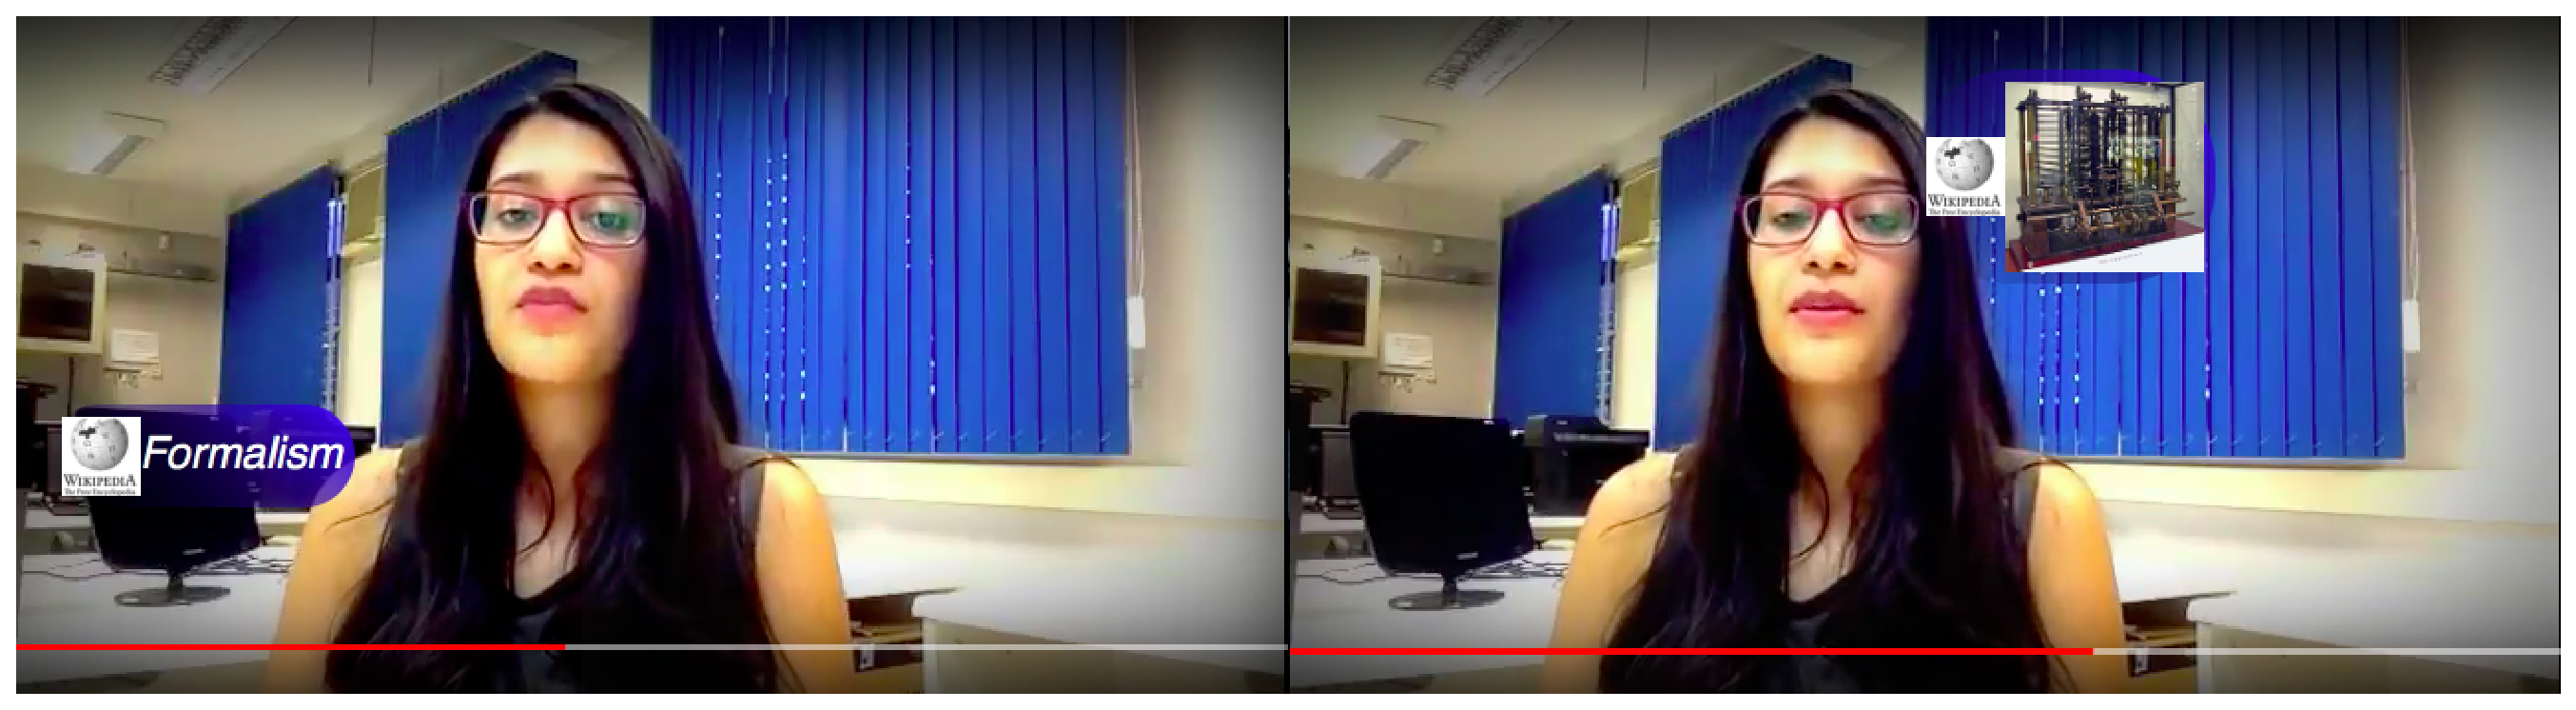
\includegraphics[scale=0.19] {figure/occlusion}}
	\caption{Occlusion Issues}
	\label{oclusion}
\end{figure}

In general, the result generated by the crowd was well adapted to convey the content intended by the author, having enriched virtually all the points that he had predicted.





















\section{Final Remarks}
	This paper presented an updated version of [REMOVED FOR BLIND REVIEW], a method for achieving a complex media annotation by running a process workflow composed of simple annotation microtasks in a cascading arrangement. Some relevant improvements were made to both the method and the framework used to support its activities.

The experiment showed that the improvements made in the method were successfully implemented, successfully generating the expected result. The contributions were obtained from a commercial crowdsourcing environment, but with a differentiated approach in which only the resources related to the workers and none of the platform resources were used. This approach ensured that both the data set used and the data collected in the contributions were stored only in our database, not the crowdsourcing platform.

It was also observed that the concept of supervised aggregation introduced in this version obtained positive results. This aggregation approach has proven to be interesting for improving the results of annotation tasks that receive open answers that need to be adjusted manually. A direct conclusion is that this approach can also be used to insert a human verification step at the end of certain aggregation activities.

The diagrams introduced considerably facilitated the creation of the workflow from the production process to the case study. In addition, a specification of the dataflow in the interfaces between the components, facilitating the planning of the distribution of the works and the information that is necessary.

The basic annotation tools distributed with the framework can be easily adapted to work with the commercial crowdsourcing platform as well as to meet the requirements of the tasks required for the experiment.

As can be seen in Figure \ref{workers}, the workers who contributed to the experiment are scattered all over the world. This ensured a heterogeneous crowd, which contributed to the operation of aggregation methods based on the wisdom theory of the crowds.
\begin{figure}[h]
	\centerline{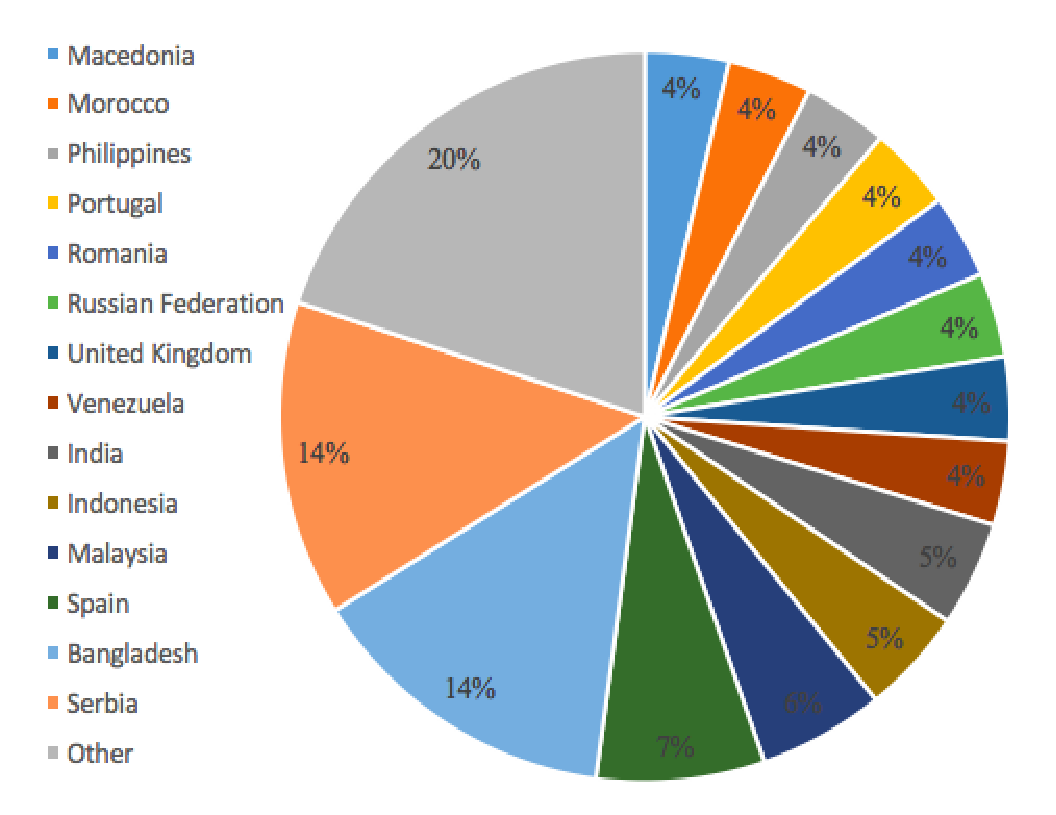
\includegraphics[scale=0.3] {figure/workers_2}}
	\caption{Workers distribution through the world.}
	\label{workers}
\end{figure}

The video enrichment process has been able to produce an interactive multimedia presentation from a simple raw video through a crowdsourcing approach. This leads to the conclusion that the updated method presented is appropriate to guide this type of project that aims to generate complex media annotations.

\subsection{Issues}
Some issues were detected in relation to the collection process. About 20\% of the contributions cannot be used because they did not meet the desired specifications or because they had invalid or malicious content. This showed that it is necessary to insert in the annotation tools some resources that induce workers to provide valid contributions. It also alerted us to the importance of giving workers clearer instructions on how to properly perform tasks.

In fact, it drew attention to the need to define criteria for the evaluation of instructions given to workers. Also came the discussion about the need for a research on whether textual instructions are really sufficient to perform any simple annotation microtasking.

\subsection{Crowds Comparison Experiment}
Another relevant discussion resulting from the observations of the results concerns the extent to which the composition of the crowd can influence the outcome.

To understand the best is not revealed, it is not a presentation method, the experiment conducted will be replicated in different scenarios:
\begin{itemize}
\item Increasing the salary of workers;
\item Choosing different contracted groups;
\item Choosing only the best workers;
\item Using a closed group with volunteers;
\item Using a group familiar with the subject treated in the video;
\item Using a group of natives in the English language.
\end{itemize}


\subsection{Next Steps}

This work is constantly improving on three different fronts: improvement of the method, improvement of the framework scenarios and application differences.

Regarding the method, the next steps include the formalization of the aggregation process, defining specific flows for automatic, supervised and manual models.

New annotation tools are being designed for the structure, which can be adapted for more tasks. In addition, a wizard is being designed to guide the creation of complex media annotation projects based on the method presented.

Some experiments are being prepared to be carried out, some of which seem especially promising:
\begin{itemize}
\item Multisensorial video annotation for mulsemedia applications.
\item Gesture segmentation in signal language video datasets.
\item Semantic approximation of idiomatic expressions in automatic translations.
\item Crowdsourcing  creation of learning object.
\end{itemize}


\begin{acks}
	The authors would like to thank FAPES, CAPES and CNPq for financial support of this research.
\end{acks}


\bibliographystyle{ACM-Reference-Format}
\bibliography{references} 

\end{document}
